\documentclass[french]{article}

\usepackage{babel}				%nécessaire pourl'option french
\usepackage[utf8]{inputenc}		%caractères accentués (entrée)
\usepackage[T1]{fontenc}		%caractères accentués (sortie)

\usepackage[top=3.5cm, left=4cm, right=4cm, bottom=3.5cm]{geometry}

\usepackage[affil-it]{authblk}	%affiliations dans le titre

\usepackage{enumitem}

\usepackage{amsmath,amssymb,amsthm}
\newtheorem{sol}{Solution}

\usepackage{graphicx}
\renewcommand{\arraystretch}{1.5}
\usepackage{multirow}

\begin{document}
\title{Installation sonore pour le brainspotting}
\author{Alice Rixte}
%\affil{Université Gustave Eiffel,\\ École Normale Supérieure Paris-Saclay}
\date{\today}
\maketitle





\section{Scenarii de projets}
\label{scenarii}

Dans tous les scenarii suivants, le thérapeute et le patient se font face à une distance de l'ordre du mètre. Dans les cas où le brainspotting visuel est combiné avec l'installation sonore, le thérapeute est décalé de 50 cm du côté opposé à sa main d'usage  par rapport à l'axe au long duquel le visage du patient est dirigé (voir Figure \ref{basic-situation}).
\begin{figure}[!h]
	\centering
	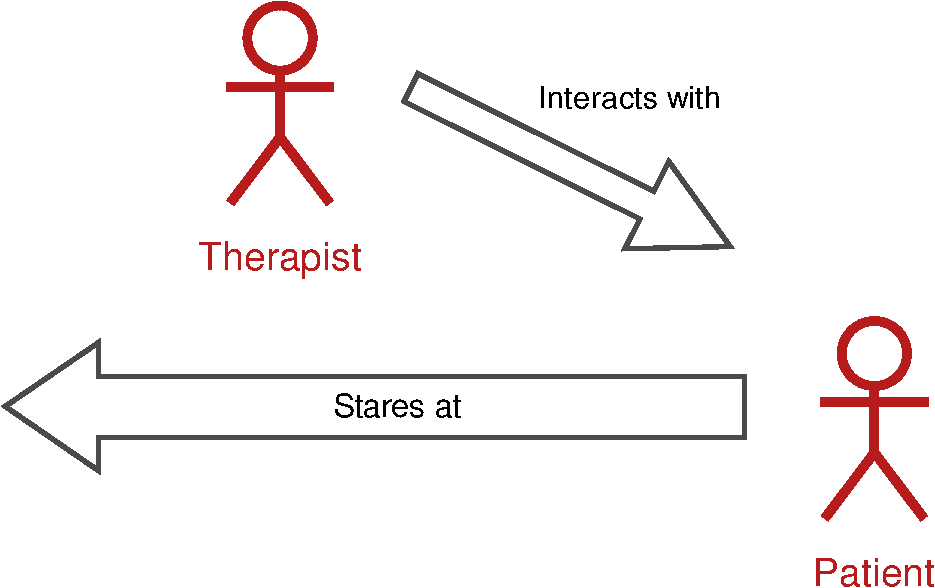
\includegraphics[scale = 0.6]{schemas/basic-situation.pdf}
	\label{basic-situation}
	\caption{Dispositif de base d'une thérapie brainspotting}
\end{figure}
\subsection{Focalisation visuelle sur un objet physique et sonore}
Pendant que le patient parle, le thérapeute concentre le regard du patient vers un object physique émettant du son. Le thérapeute peut agir depuis sa position sur la localisation de cet objet physique ainsi que sur sa distance.
\paragraph{Variante a)}
Le thérapeute peut détacher ou rattacher la localisation de l'objet sonore à celle de l'objet physique. Le thérapeute peut alors maîtriser à la fois la position de l'objet visuel et celle de l'objet sonore.
\paragraph{Variante b)}
La localisation sonore est moins précise que la localisation visuelle et l'objet visuel et sonore sont situés dans la même direction.
\subsection{Focalisation visuelle sur un objet sonore}


Pendant que le patient parle, le thérapeute concentre le regard du patient vers un object sonore immatériel. Le thérapeute peut agir depuis sa position sur la localisation de cet objet ainsi que sur le distance. Le visage du patient est toujours touné dans la même direction, seuls ses yeus bougent. L'objet sonore se situe donc dans le cône de vision du patient (voir Figure \ref{conic-situation}).

\begin{figure}[!h]
	\centering
	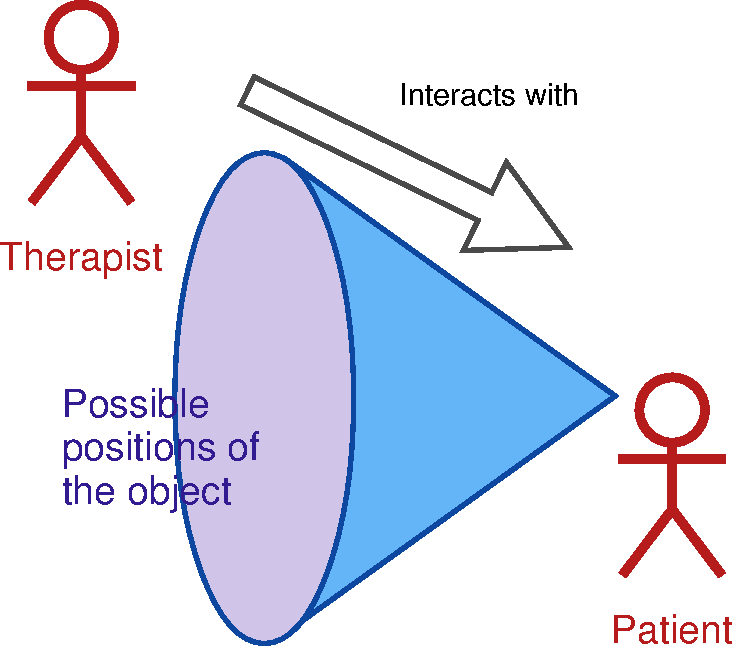
\includegraphics[scale = 0.6]{schemas/conic-situation.pdf}
	\label{conic-situation}
	\caption{Objet dans le champ visuel}
\end{figure}

\paragraph{Variante b)}
L'objet sonore peut se trouver derrière le patient. Celui-ci a toujours la consigne de regarder dans la direction de l'objet sonore. On peut par exemple lui suggérer de regarder à l'exact opposé de la source sonore. Dans ce cas, l'objet sonore peut se trouver dans deux cônes opposés.

\begin{figure}[!h]
	\centering
	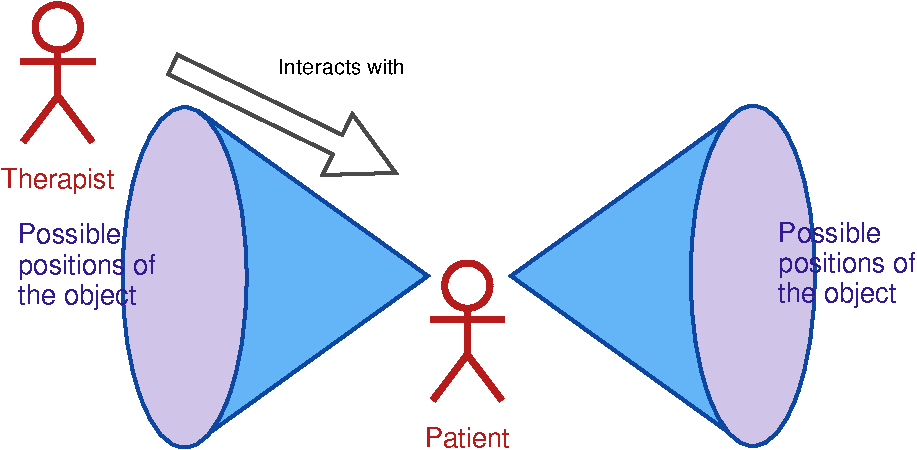
\includegraphics[scale = 0.7]{schemas/double-conic-situation.pdf}
	\label{double-conic-situation}
	\caption{Objet dans le champ visuel et son opposé}
\end{figure}



\subsection{Focalisation sonore}
Pendant que le patient parle, le thérapeute concentre l'attention du patient vers un object sonore immatériel. Ici, le patient ne suit pas des yeux la localisation de l'objet mais essaie de se la représentermentalement. Le thérapeute peut contrôler la localisation du point sonore.

\paragraph{Variante a)} Le patient doit suivre des yeux un point dans l'espace dont la localisation est décorellée de celle de l'objet sonore.

\paragraph{Variante c)} Le patient a les yeux fermés
\paragraph{Variante ac)} Le patient suis l'objet sonore des yeux malgré ses paupières fermées.

\subsection{Thérapie portable}
Dans son activité, le thérapeute a besoin d'utiliser son installation de brainspotting sonore dans divers lieux de pratique professionnelle. Il doit donc avoir la possibilité de transporter l'installation simplement.

\subsection{Autothérapie}
Dans ce scénario, le patient utilise l'installation seul. Il a donc à la fois le rôle du thérapeute et celui de patient. Il peut donc piloter  la localisation du son lui-même. Il peut notamment vouloir fermer les yeux et continuer le pilotage du son malgré cela.


\section{Classification des scenarii}
À partir des différents scenarii de projets que listés en Section \ref{scenarii}, on peut généraliser l'usage de la manière suivante : 

\paragraph{Scenario générique} 
Le patient focalise son attention sur des objets qu'il peut localiser pendant qu'il fait appelle à sa mémoire et au langage. Le nombre d'objets est indéfini. La présence d'un thérapeute est optionnelle. 

Les acteurs sont alors le patient et le.a potentiel thérapeute. Le premier acteur (patient) peut faire deux actions : 
\begin{itemize}[label={\textbullet}]
	\item Modifier la position spatiale d'un des objets
	\item Focalizer son attention sur un ou plusiurs objets
\end{itemize}
Le second acteur peut faire une unique action : 
\begin{itemize}[label={\textbullet}]
	\item  Modifier la position spatiale d'un des objets
\end{itemize}

\begin{table}[h]
	\begin{tabular}
		{|c|p{0.1\textwidth}p{0.1\textwidth}p{0.1\textwidth}
		p{0.1\textwidth}p{0.1\textwidth}p{0.1\textwidth}|}
		\hline
		Nature                                & \multicolumn{3}{|c|}{Visuel}     &
		                                      & \centering Sonore                &                       \\
		\hline
		Tangibilité                           &                                  & \centering Matériel &
		                                      & \multicolumn{3}{|c|}{Immatériel}                         \\
		\hline
		\multirow{4}{*}{ Localisation }       &
		\multicolumn{2}{|c|}{Cône}            &
		\multicolumn{2}{|c|}{2 cônes opposés} &
		\multicolumn{2}{|c|}{Espace 3D}                                                                  \\
		\cline{2-7}
		                                      & \multicolumn{3}{|c|}{Précise}
		                                      & \multicolumn{3}{|c|}{Diffuse}                            \\
		\cline{2-7}
		                                      & \multicolumn{3}{|c|}{Continue}
		                                      & \multicolumn{3}{|c|}{Discrète}
		\\
		\cline{2-7}
		                                      & \multicolumn{3}{|c|}{Mobile}
		                                      & \multicolumn{3}{|c|}{Immobile}
		\\
		\hline
		Contrôle                              &
		\multicolumn{2}{|c|}{Physique}        &
		\multicolumn{2}{|c|}{Télécommandé}    &
		\multicolumn{2}{|c|}{Autonome}
		\\
		\hline
		Synchronisation  & \multicolumn{3}{|c|}{Synchronisé}
		& \multicolumn{3}{|c|}{Non synchronisé}\\
		\hline
	\end{tabular}
	\caption{Caractéristiques de l'objet de la focalisation du patient}
	\label{objet-carac}
\end{table}

\paragraph{}
La plupart des variantes définies en Section \ref{scenarii} peuvent être résumées par différents choix sur les caractèristiques des objets sur lesquels se focalise le patient (voir Table \ref{objet-carac}) ainsi que par des limitations sur les mouvements du patients (immobile / peut tourner la tête / peut se déplacer). Dans le cas des mouvements du patients, on obtient une action supplémentaire pour le patient (bouger la tête / se déplacer).



\section{Solutions techniques}

On s'intéresse ici à générer un objet \emph{sonore} localisable dans l'espace.

\subsection{Patient et thérapeute en mouvement}

Une première solution consisterait en un casque audio stéréo. Localiser les sons via un système binaural est relativement efficace. Malgré cela, cette localisation manque de précision, du fait d'une morphologie de la tête différente chez chaque être humain et du rôle que le lobe de l'oreille joue dans la localisation des sons. Nous ne nous intéresserons donc pas à cette solution dans ce projet. Le fait que le patient puisse se déplacer ou tourner la tête nécessite des capteurs tels que ceux que l'on peut trouver notamment dans les casques de réalité virtuelle.
\begin{sol}[Casque de réalité virtuelle]
	Utiliser un casque de réalité virtuelle sans nécessairement utiliser la composante visuelle.
\end{sol}

J'opterai donc ici pour des sources sonores détachées du patient. La question du type de source entre en jeu : si le patient peut se déplacer, il devient nécessaire d'obtenir une source sonore omnidirectionnelle. Dans ce cas, la source sonore et l'objet de focalisation ne font qu'un. Une solution simple et efficace entre en jeu : le thérapeute tient dans sa main un haut-parleur portatif et le déplace à sa guise.
\begin{sol}[Haut-parleur amovible]
	\label{hp-amovible}
	Le thérapeute déplace un haut-parleur portatif.
\end{sol}

Les désavantages de la solution \ref{hp-amovible} sont les suivants : 
\begin{itemize}[label={\textbullet}]
	\item L'objet \emph{sonore} est visualisable et \emph{matériel} : il ne fait qu'un avec la source sonore.
	\item On ne peut avoir qu'un unique objet \emph{sonore}.
\end{itemize}

Pour libérer les mains du thérapeute, on imagine donc que  la ou les sources sonores puisse être fixés sur des supports. On pourrait alors imaginer un moteur déplace ces sources sonores, ce qui serait extrêmement coûteux mais néanmoins intéressant.

\begin{sol}[Sources sonores motorisés]
	On utilises une ou plusieurs sonors qui se déplacent physiquement dans l'espace.
\end{sol}

Si toutefois la position du haut parleur est fixée, la localisation se fera nécessairement de manière \emph{discrète}. En effet, si l'on souhaitais ajouter  des effets de stéréos entre deux sources,  on n'aurait aucun moyen a priori de savoir quelle source est plutôt à droite du patient et quelle source est plutôt à gauche. 

\begin{sol}[Sources sonores fixes]
	\label{solSrcFixe}
	L'idée est de placer plusieurs sources sonores dans l'espace de thérapie. Une illusion de mouvement peut-se créer en passant d'une source sonore à l'autre.
\end{sol}

\section{Patient assis}

L'immobilité du patient permet non seulement d'utiliser de ne plus se contraindre à des sources sonores omnidirectionnelles mais permet également la création d'une illusion de continuité dans la positions des objets sonores en adaptant la Solution \ref{solSrcFixe}. En effet, il est standard en stéréo par exemple de virtuellement centrer un objet sonore en envoyant l'émission sonore de l'objet avec le même volume à gauche et à droite. On peut ainsi créer un segment continu virtuel entre deux hauts parleurs (voir Figure \ref{stereo-localization})

\begin{figure}[!h]
	\centering
	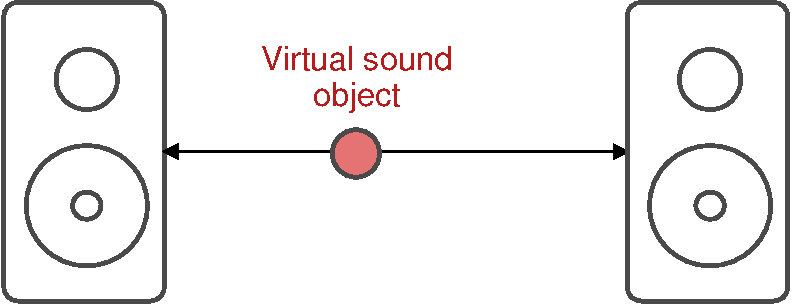
\includegraphics[scale = 0.7]{schemas/stereo-localization.pdf}
	\caption{Objet dans le champ visuel et son opposé}
	\label{stereo-localization}
\end{figure}



\end{document}